\chapter{Technical Background}\label{chapter:technicalBackground}

This chapter provides an overview of most of the techniques, frameworks, and libraries related to the thesis, including the Robot Operating System ROS, used Lidar sensors, Gazebo, Turtlebo3 models, RViz, OpenCV, Pytorch, PointNet, and different models used for the representation of colors and calculating of their differences.

\section{Robot Operating System}

%(TODO citation) 
Robot Operating System, shortly ROS is a popular open-source framework commonly used by many researchers and robot developers. This framework allows easy launch, deployment, and communication between different modules as standalone services that create a final complex system. This modularity permitted the creation and easy application of various tools and libraries like Gazebo, RViz, or rqt (TODO references), together with custom services. Furthermore, the ROS allows an easy spread of one system among more devices, allowing an easy run of some services directly on the robot and other services on the central computer, without almost any accessive work.\par
Another significant advantage of the ROS's modularity is that you can exchange the robot simulator with the real robot and sensors without touching the rest of the system. Furthermore, you can record and replay the entire system's messages during its run, allowing easy reproducibility of any experiment.\par
The official languages of the ROS are C++ and Python, but there are also inofficial tools that allow writing services for ROS in other languages, like, for example, LISP or Swift. (TODO references)\par
The following subsections briefly introduce some of the essential ROS features.

\subsection*{Roscore}

Roscore is a service that must be executed before running any Node of the ROS system. This service will automatically start all the essential services for the ROS running, like logging service, parameter server, and ROS master. Therefore, the running roscore service is necessary for ROS nodes to communicate.

\subsection*{ROS Node}

Ros Nodes are a crucial concept of the whole system. Single Node represents a standalone service that can process data received from other ROS Nodes, sensors, or users and send them to the other Nodes or directly to the user or system actors. The entire application usually consists of many ROS Nodes that communicate using ROS topics, services, etc.

\subsection*{ROS message}

Messages are the most common way of communication between several ROS Nodes. These messages are transmitted between the Nods via ROS topics. The ROS message, typically stored in the .msg file, describes a format that the data transmitted on a particular ROS topic must fulfill and tells the ROS Node how to represent the received data.\par
According to the convention, most messages start with the Header part, containing the message sequence number, timestamp, and frame id. However, this header is optional and is not present in all commonly used messages.

\subsection*{ROS topic}

ROS topics are named buses, serving for message exchange between the Nodes. One or more Nodes can publish messages or subscribe to each ROS topic and receive all published messages. The publishing and subscribing processes work anonymously, which means that the publisher does not know if the message was read by only one or more or any Node, and receivers do not know which node published the particular message unless it's part of the sent data.\par
Every topic is strongly connected with a particular message type, so every message published on the same topic must have the same format.

\subsection*{Roslaunch}

Roslaunch is a tool allowing the launch of multiple ROS Nodes with a single command based on an XML configuration. This tool also supports setting different parameters that can be set while starting the process and passed to the particular Nodes or put on the Parameter Server. Furthermore, this tool allows renaming specified topics without the need to tell any information to the publishing Nodes.

\subsection*{ROS package}

ROS packages help to organize the ROS software. The package can contain ROS Nodes, libraries, datasets, configuration files, etc. The goal of the ROS package is to pack together connected ROS Nodes and other tools that together create some meaningful tool, program, or library. These packages allow easy publication, deployment, installation, and integration of the third-party components into custom programs or systems.

\subsection*{Rosbag}

Rosbag is a command line tool for recording and replaying the data exchanged between Nodes during the program run. This tool can record all messages published on all or only specified ROS topics without affecting the running system. These messages can be later replayed, which allows excellent reproducibility of all program runs and further optimization, improvement, and testing under the same conditions.\par
Particularly researchers with this tool record all data from the sensors while running experiments and publish them on the internet for later experiment reproduction or further development.

\subsection*{Catkin}

Catkin is a collection of CMake macros and Python scripts commonly used for the ROS development and building of ROS Nodes and packages. Even if catkin is not the official part of ROS, it is a widely used tool among the ROS community.

\section{Gazebo}

%(TODO ref)
Gazebo is a famous open-source 3D-simulation tool supporting robot simulation in complex 3D environments, including realistic physics, like gravity, friction, collisions, light reflections, etc. These environments can also change over time, which allows adding pedestrians, moving cars, or other non-stationary objects to the simulation.\par
Furthermore, Gazebo supports various types of sensors, especially HD-Camera, 3D or 2D Lidar, IMU, etc., or several plugins for the robot control. This tool also provides an interface fully compatible with ROS, which makes it a perfect simulation tool for this thesis.

\section{Turtlebot3}

Turtlebot3 offers open-source mobile robots commonly used in robotics research and development. The Turtlebo3 provides two different models, Burger and Waffle-Pi, that are fully compatible with the Gazebo simulator and contain all software necessary for the robot control and simulation. These models are also easily extensible and allow adding new kinds of sensors.

\section{RViz}

RViz is a ROS graphical interface, allowing the visualization of the information published for many different available topics. Particularly, this tool is commonly used for the real-time visualization of the data received from various sensors, generated maps, landmarks, detected objects, etc.

\section{OpenCV}

%(TODO ref)
OpenCV is an open-source computer vision library available for C++ and Python. This library contains many real-time image and video processing tools, from simple transformations to feature extraction and matching or object recognition.

\section{Pytorch}

%(TODO ref)
Pytorch is a python open-source machine learning framework based on the Torch library. This framework is commonly used in the area of machine learning. It contains many tools for modeling Neural Networks, several training algorithms, tools for datasets preparation, advanced matrix operations tools, etc. Furthermore, because of the CUDA support, this framework allows running most of the calculations on the GPU, which can significantly speed up the training process of most models.

\section{PointNet}

PointNet [TODO ref] is a deep neural network widely used for point cloud processing by many applications. This network can extract the feature vector from any point cloud, invariant to the order of the points and the rotation of the scene that the input cloud represents. Furthermore, the input size in terms of the number of points can vary for each input. There is available a C++ implementation [TODO ref] of the network, as well as a Python implementation in TensorFlow [TODO ref] or PyTorch [TODO ref] version.\par
Except for the feature extraction, the implementations of the PointNet network also include additional networks for scene segmentation and object classification based on the extracted feature vector from the PointNet network. Furthermore, all required learning and dataset preparation algorithms are also included.

\section{Color Models}

There are many different ways to represent a single color on a computer. Except for the well-known RGB representation, there are many different other representations with distinct advantages. Lab [TODO refs] representation is for the work the most interesting because it allows easy color difference computation, using CIE76 [TODO ref] and CIE2000 [TODO ref] that correspond in the best way to the difference told by humans.\par
Similarly, as in an RGB format, the colors are represented using three different components, L, a, and b. The L part stands for lightness and means how light or dark the color is. The a and b components represent the balance between two different colors. The a part describes the balance between green and magenta, and the b part represents the balance between blue and yellow. Even if this color scheme can describe the whole space of colors, the colors visible by human eyes are located in a sphere, displayed in Figure \ref{fig:labscheme}.

%https://www.researchgate.net/figure/CIELab-1976-after-Figure-1-from-SantAnna-et-al-2013-602_fig4_311426707
\begin{figure}[htpb]
    \centering
    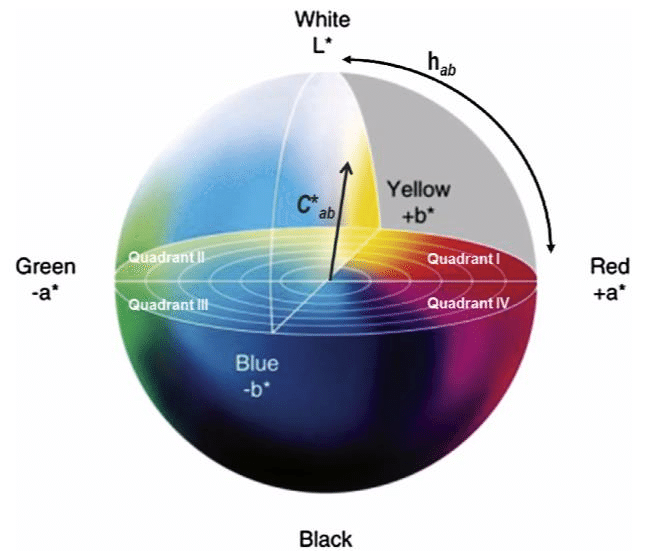
\includegraphics[width=0.8\textwidth]{Lab.png}
    \caption{Visualization of an Lab color representation [TODO ref]} \label{fig:labscheme}
\end{figure}
